\documentclass[a4paper,11pt,eval]{nsi} 
\usepackage{fontawesome5}

%\pagestyle{empty}


\newcounter{exoNum}
\setcounter{exoNum}{0}
%
\newcommand{\exo}[1]
{
	\addtocounter{exoNum}{1}
	{\titlefont\color{UGLiBlue}\Large Exercice\ \theexoNum\ \normalsize{#1}}\smallskip	
}



\begin{document}



\textcolor{UGLiBlue}{Mercredi 26/02/2025}\\
\classe{\terminale Comp}
\titre{Évaluation-bilan 4}
\maketitle
\begin{center}
	Calculatrice autorisée. Toutes les réponses doivent être justifiées.
\end{center}

%\vspace*{1cm}


\dleft{11.5cm}{
    \exo{}\bareme{4 pts}\\
    Dans une kermesse, on fait tourner la roue de loterie équilibrée ci-contre où tous les secteurs ont le même angle.\\
    Le joueur gagne le nombre de points indiqué par le secteur désigné par la flèche.\\
    $X$ est la variable aléatoire qui donne le gain du joueur.
}
{
    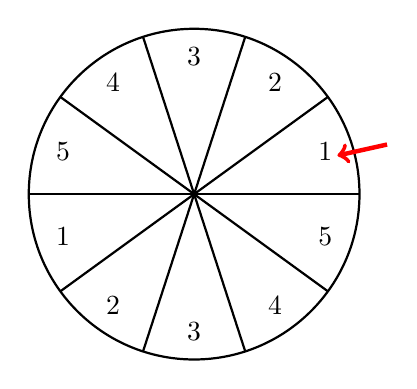
\begin{tikzpicture}[scale=.7]
        \foreach \i in {1,...,10} {
            \draw[thick] (0,0) -- ({36*\i}:3);
            %\node at ({30*(\i-0.5)}:2.5) {\i};
        }
        \foreach \i in {1,2,3,4,5} {
            \node at ({36*(\i-0.5)}:2.5) {\i};
            \node at ({36*(\i+4.5)}:2.5) {\i};
        }
        \draw[thick] (0,0) circle(3);
        \draw[->, ultra thick, red] (3.5,.9) -- (2.6,.7); % Ajout de la flèche
    \end{tikzpicture}
}
\begin{enumerate}
    \item Quelle est la loi de probabilité suivie par $X$ ?
    \item Combien de points un joueur peut-il espérer gagner en moyenne lors d'une partie ?
    \item Pour pouvoir tourner la roue, le joueur doit payer 1 euro. Un point rapporte 0,30 €. Le jeu est-il équitable?
\end{enumerate}
\carreauxseyes{16.8}{11.2}

%\vspace*{.5cm}


\dleft{13.5cm}{
    \exo{ Au casino}\bareme{6 pts}\\
    On suppose que la probabilité de gagner une partie à une machine à sous est de 0,001.\\
    On suppose que toutes les parties sont indépendantes et on appelle $X$ la variable aléatoire qui donne le rang de la première partie gagnée lorsqu'on joue plusieurs parties successives.\\
}
{\includegraphics[width=3cm]{casino-161438_1280.png}}
\begin{enumerate}
    \item Quelle est la loi de probabilité suivie par $X$ ? Préciser le ou les paramètres.
    \item En combien de parties peut-on espérer gagner pour la première fois avec cette machine à sous ?
    \item Calculer $P(X>500)$ puis interpréter ce résultat.
    \item La mise de cette machine à sous est de 2 €.\\
    Quelle est la probabilité que l'on gagne avant de ne plus avoir d'argent si on dispose de 2000 € ?
\end{enumerate}
\carreauxseyes{16.8}{17.6}


\dleft{11cm}{
    \exo{ Planche de Galton}\bareme{5 pts}\\
    Dans une fête foraine, on fait glisser un palet le long d'une planche cloutée comme ci-contre.\\
    À chaque étage, le palet rencontre un clou et va à gauche ou à droite avec la même probabilité. Après 4 étages, le palet arrive dans un des cinq bacs de réception numérotés de 0 à 4.}
{
    \begin{tikzpicture}
        % Dessiner les étages
        \foreach \i in {0,1,2,3} {
            \foreach \j in {0,...,\i} {
                \filldraw[black] (\j-\i/2, -\i) circle (2pt);
                % Ajouter des flèches à droite et à gauche de la bille
                \draw[->, thick] (0.1+\j-\i/2, -0.1-\i) -- (0.3+\j-\i/2, -0.5-\i);
                \draw[->, thick] (-0.1+\j-\i/2, -0.1-\i) -- (-0.3+\j-\i/2, -0.5-\i);
            }
        }
        
        % Dessiner les lignes de sortie
        \foreach \i in {-1,0,1,2,3,4} {
            \draw[thick] (\i-1.5, -3.5) -- (\i-1.5, -4.5);
        }
        \foreach \i in {0,1,2,3,4} {
            \node[UGLiBlue] at (\i-2,-4) {\i};
        }
        
        % Dessiner les bords de la planche
        \draw[thick] (-.5, 0.5) -- (-2.5, -3.5);
        \draw[thick] (.5, 0.5) -- (2.5, -3.5);
        \draw[thick] (-2.5, -4.5) -- (2.5, -4.5);
        
        % Ajouter une bille au sommet
        \filldraw[UGLiBlue] (0, 0.5) circle (5pt);
        
    \end{tikzpicture}
}
\begin{enumerate}
    \item \begin{enumalph}
        \item  Dans quel bac le palet arrivera-t-il s'il va à gauche puis à droite, puis à gauche, puis à gauche ?
        \item Dans quel bac le palet arrivera-t-il s'il va à droite puis à droite, puis à gauche, puis à droite ?
    \end{enumalph}
   \item On appelle $X$ la variable aléatoire qui donne le numéro du bac de réception du palet.
   \begin{enumalph}
        \item Expliquer pourquoi la loi de probabilité de $X$ est une loi binomiale dont on précisera les paramètres $n$ et $p$.
        \item Calculer l'espérance de $X$.
        \item Le gros lot est gagné si le palet arrive dans le bac 4.\\
        Quelle est la probabilité de gagner le gros lot ?
    \end{enumalph}
\end{enumerate}
\carreauxseyes{16.8}{14.4}

\exo{ Loi de refroidissement de Newton}\bareme{7 pts}\\
Une tasse de café est servie à une température initiale de 80°C. On la laisse refroidir dans une pièce à température ambiante de 10°C.\\
On va étudier à l'aide d'une suite le refroidissement du café en appliquant la loi de Newton.\\

Pour tout entier naturel $n$, on note $t_n$ la température du café (en °C) au bout de $n$ minutes.\\
On a ainsi $t_0=80$. Entre deux minutes consécutives $n$ et $n+1$, on a $t_{n+1}-t_n=-0,2(t_n-10)$.
\begin{enumerate}
    \item Conjecturer d'après le contexte le sens de variation de la suite $(t_n)$.
    \item Montrer que, pour tout entier naturel $n$, on a $t_{n+1}=0,8t_n+2$.
    \item Exprimer $t_n$ en fonction de $n$.
    \item Déterminer la limite de la suite $(t_n)$.
    \item \faCalculator \hspace*{.2cm} Combien de temps faut-il pour que la température du café soit inférieure à 20°C ?
\end{enumerate}

\carreauxseyes{16.8}{16.8}
\end{document}